% Created 2017-12-23 Sat 22:14
% Intended LaTeX compiler: pdflatex
\documentclass[11pt]{article}
\usepackage[utf8]{inputenc}
\usepackage[T1]{fontenc}
\usepackage{graphicx}
\usepackage{grffile}
\usepackage{longtable}
\usepackage{wrapfig}
\usepackage{rotating}
\usepackage[normalem]{ulem}
\usepackage{amsmath}
\usepackage{textcomp}
\usepackage{amssymb}
\usepackage{capt-of}
\usepackage{hyperref}
\usepackage{tikz}
\author{scott}
\date{\today}
\title{}
\hypersetup{
 pdfauthor={scott},
 pdftitle={},
 pdfkeywords={},
 pdfsubject={},
 pdfcreator={Emacs 25.3.1 (Org mode 9.1.4)}, 
 pdflang={English}}
\begin{document}

\tableofcontents

First execute the second code block, to define the convenience macro
and to set the required new variables in ob-latex.el.  Then export to
HTML and to pdf to see the tree exported as an SVG image and as
embedded tikz respectively.

\section{Tikz test}
\label{sec:org5ea408c}
Here's a tree, exported to both html and pdf.

\usetikzlibrary{trees}
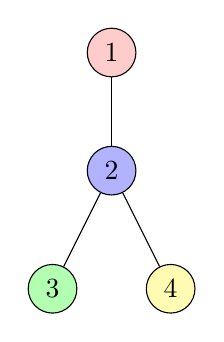
\begin{tikzpicture}
  \node [circle, draw, fill=red!20] at (0,0) {1}
  child { node [circle, draw, fill=blue!30] {2}
    child { node [circle, draw, fill=green!30] {3} }
    child { node [circle, draw, fill=yellow!30] {4} }};
\end{tikzpicture}
\end{document}